\section{Auvi}

\subsection{Programm} % AuVi
Um Verwechslungen zu verhindern benennen wir das Programm, welches wir unter AuVi entwickelt haben ,,\vs ''. Das steht für Visualisierung System und ist in verschiedenen Versionen lauffähig.
Die Aufgabe von \vs\ ist es auf eine Datenquelle zuzugreifen und nach abgespeicherten Parametern die Rohdaten in Grafiken umzuwandeln.
Dabei wird von uns sehr viel Wert darauf gelegt, dass das Erstellen der Grafiken möglichst abstrakt behandelt wird, damit der Nutzer sehr großen Einfluss auf das Design und den Inhalt der Grafiken nehmen kann.

\subsection{Meteorologie} % AuVi

\subsubsection{Prognosetheorie} % AuVi Meteorologie
Die Meteorologie gehört zu den Naturwissenschaften.
Sie liefert die Voraussetzungen um eine Wettervorhersage erstellen zu können.
Unter einer Wetterprognose versteht man die Vorhersage eines Zustands der Atmosphäre zu einem bestimmten Zeitpunkt an einem bestimmten Ort oder in einem bestimmten Gebiet.
Es wird nicht nur das Wetter in Bodennähe betrachtet, sondern auch Wettererscheinungen in höheren Schichten der  Erdatmosphäre.
\\
Das Wetter lässt sich durch entsprechende Naturgesetze beschreiben. Das ist für die Prognose essentiell wichtig.
Der Grundgedanke einer solchen Prognose besteht darin, aus einem bereits vergangenen und dem aktuellen Zustand der Atmosphäre einen Zustand in der Zukunft abzuleiten.
Dazu werden die bekannten physikalischen Regeln angewendet.
In mathematischer Hinsicht werden diese physikalischen Regeln von nichtlinearen Gleichungen beschrieben.
Das bedeutet, dass bereits die kleinste Änderung im Ausgangszustand das Ergebnis der Rechnung relativ groß verändern kann.%[1]

\subsubsection{Prognosen per Hand} % AuVi Meteorologie
Was muss man über die aktuelle Situation wissen um per Hand eine Prognose zu erzeugen?
Es gibt einen Unterschied zwischen der manuellen oder auch synoptischen Wettervorhersage und einer numerischen Wettervorhersage.
In der synoptischen Meteorologie ist ein System aus Beobachtungsstationen nötig, die gleichzeitig Wetterbeobachtungen nach einem einheitlichen Verfahren durchführen.
Die Stationen messen unter anderem Parameter wie:
Luftdruck, Luftdruckänderung während der letzten drei Stunden, Lufttemperatur, Windrichtung, Windgeschwindigkeit, Taupunkt, Wolkenart, Höhe der Wolkenuntergrenze, Bedeckungsgrad, Sichtweite, Niederschlagsmenge und Niederschlagsart.
Es wird zwischen Bodenbeobachtungsstationen, die Daten in der Nähe der Bodenoberfläche sammeln und aerologischen Beobachtungsstationen, die Daten aus bis zu 30km Höhe liefern unterschieden.
Es werden auch Daten von mobilen Messstationen, wie Bojen und Flugzeugen verwendet.
Wettersatelliten und Fernerkundungssystem (wie Wetterradar, Blitzortungssysteme, LIDAR, SODAR) können auch als Datenquelle dienen.
Die gesammelten Daten, die den Wetterzustand zu einem bestimmten Zeitpunkt beschreiben, werden in Wetterkarten eingetragen.
Mit Hilfe der eingetragenen Daten werden die Wetterverhältnisse analysiert und Wettervorhersagen erstellt.
Zusätzlich dazu werden die gesammelten Daten von numerischen Vorhersagemodellen als Ausgangszustand verwendet. %[2]
\\
Numerische Wettervorhersagen sind rechnergestützt.
Der Zustand der Atmosphäre zu einem späteren Zeitpunkt wird aus dem Zustand der Atmosphäre zu einem gegebenen Anfangszeitpunkt berechnet.
Dabei werden relevante Gleichungen numerisch gelöst
(Navier-Stokes-Gleichung, thermische Zustandsgleichung idealer Gase, erster Hauptsatz der Thermodynamik, Kontinuitätsgleichung).
Mit diesen Gleichungen werden Vorgänge, wie zum Beispiel Wolkenbildung, Niederschläge, Bildung von Hoch-  und Tiefdruckgebieten und Wind beschrieben.
Diese Vorgänge können je nach Luftdruck, Temperatur, Windgeschwindigkeit und Luftfeuchtigkeit auftreten.
Da diese Gleichungen jedoch nicht eindeutig lösbar sind, kann es nur zu Näherungswerten kommen.
Diese mathematischen Näherungen benötigen sehr viel Rechenleistung,
weswegen auf die Leistungsfähigkeit von Supercomputern zurückgegriffen wird.
Bei solchen numerischen Vorhersagemodellen wird das betrachtete Gebiet in Gitterzellen unterteilt.
Für jeden Punkt werden dann die Parameter errechnet.
Relevante physikalische Größen sind vor allem Temperatur, Luftdruck, Dichte, Windrichtung und Windgeschwindigkeit.
Es wird zwischen Global- und Lokal- oder Ausschnittsmodellen unterschieden.

\subsubsection{Voraussetzung für Wetterprognosen} % AuVi Meteorologie
Um Wetterprgnosen erstellen zu können, braucht man gewisse Ausgangswerte.
Die Ausgangsdaten bestehen aus Werten,
die an dem Punkt zu einem früheren Zeitpunkt gemessen wurden.
Die Entwicklung der verschiedenen Wettergrößen wird durch Formeln errechnet.
Diese Berechnung benötigt, wie oben schon erwähnt, eine enormer Rechenleistung.
Deswegen ist man für die Vorhersage von Wetterverhältnissen auf die Hilfe eines leistungsfähigen Computers angewiesen.
Die entstandenen Modellergebnisse bilden die Basis, und können nun von Prognostikern interpretiert und beurteilt werden.
Die Prognostiker können die Modelle anhand von aktuell gemessenen Werten oder Bildern einer Webcam überprüfen und eine Vorhersage formulieren.
Dabei spielen das Wissen und die Erfahrungen der Prognostiker eine große Rolle.
Die Genauigkeit einer Wettervorhersage ist von der Stabilität der Wetterlage abhängig.
Bei wechselhaftem Wetter ist die Vorhersage deutlich schwieriger und komplizierte als bei stabilen Wetterlagen.
Die Länge der Prognose spielt auch eine Rolle.
Es macht einen Unterschied,
ob man nur die Prognose für den nächsten Tag,
oder ob man die Prognose für die nächste Woche haben möchte.
Letzters ist deutlich schwieriger und somit auch weniger zuverlässig.

\subsection{Datenquellen} % AuVi

\subsubsection{Quellenvergleich} % AuVi Datenquellen
Da wir nun dargestellt haben, dass es für uns nicht möglich ist unsere eigenen Daten zu generieren, zeigen wir nun welche Quellen die benötigten Daten zur Verfügung stellen.
Der Nutzer kann selbst zwischen den verschiedenen Datenquellen wählen, die angeboten werden.
Die angebotenen Datenquellen können über die GUI und die Konsole gewählt werden.

Wir werden über eine GUI\footnote{\textit{Graphical User Interface} engl. IT. für grafische Benutzeroberfläche} dem Nutzer anbieten zwischen verschiedenen Datenquellen zu wählen.
Diese werden wir auch statistisch vergleichen.
Grafik: Übersicht über Quellen (Alle die direkt über das Programm angeboten werden)
Programm kann um weitere erweitert werden.
Auswahl NOAA, GFS.\cite{noaa}
% NOTE Viel mehr Parameter, Daten bei NOAA oc DWD
% Siehe andere Quellen


\subsubsection*{Wetterdienst} % AuVi Datenquellen
% TODO Grafik: Diagramm der Genauigkeit (Dafür Tabelle, Swenja)
Der Deutsche Wetter Dienst steht unter dem Bundesministerium für Verkehr und digitale Infrastruktur. \cite{bmvi}
Der DWD bietet ebenfalls Wetterdaten an, die allerdings kostenpflichtig sind.
Das Angebot ist unterteilt in ,,Aktuelles Wetter, Vorhersagen'' und ,,Vergangenes Wetter, Klimainfos''.
Im ersten Bereich gibt es zum Beispiel den Unterpunkt Seewetter.
Es wird ein Kurzfrist-Seewetterbericht, Küstenwetter in Zeitreihenform und ein Mittelfrist-Seewetterbericht für 48h für je 2,50 Euro angeboten.
Wenn man aus dieser Quelle alle zwei Tage eine Wetterprognose bezieht - welche im Parameter stark eingeschränkt ist - belaufen sich die Kosten auf ungefähr $\approx 230$ Euro Diese Wetterdaten können dann zum Beispiel für die Seefahrt genutzt werden.
Ein anderer Unterpunkt ist Flugwetter.
Dort gibt es Einjahresangebote für circa 80 Euro und Lehrfilmreihen für circa 150 Euro.
Diese dienen als Dokumentation.
Die Nutzer dieser Leistungen sind vermutlich größere Flughäfen.
Ein weiterer Bereich in dem Jahresabos und Monatsabos angeboten werden, ist Agrarwetter.
Die Kosten dafür belaufen sich auf 20 bis 120 Euro.
Der wohl interessanteste Unterpunkt ist Straßenwetter.
Da werden einmalige Informationen für allgemeine Wettervorhersagen für Straßen (4,40 Euro),
für detaillierte Gebietswettervorhersagen für Straßen (4,40 Euro) und für Straßenwettervorhersagen für eine Stadt (5 Euro) dargeboten.\\
Im zweiten Bereich gibt es die genaueren Eingrenzungen ,,Deutschland - Allgemein'', ,,Deutschland - Speziell'' , ,,Global'' und ,,Geburtstagswetterkarte''.
\cite{dwd-shop}
Diese Daten sind für uns allerdings nicht relevant, weil sie in der Vergangenheit liegen.\\
Da diese Quelle sich auf lange Zeit für uns als zu kostspielig herausgestellt hätte,
und auch die Datenmenge nicht für jeden Punkt der Erde definiert ist,
war für uns frühzeitig klar, dass wir uns eine alternative Quelle suchen mussten.

\subsubsection*{NOAA Global Forecast System} % AuVi Datenquellen
Das Global Forecast System (GFS)  ist ein Modell, das mathematisch Parameter errechnet.
Es ist also ein numerisches Vorhersagemodell.
Die dazu benötigten Daten bezieht es aus einem Netz von Wetterstationen,
die sowohl an Land als auch im Wasser und in der Luft Messungen durchführen.
Mit diesen gemessenen Daten werden mithilfe von geophysikalischen Gesetzen weitere Daten errechnet.
So wird in einem Abstand von 13,5km je ein Wert ermittelt.
Diese Daten werden als große Datensätze kostenfrei auf der Webseite \link{http://mag.ncep.noaa.gov/} \cite{ncep}  zur Verfügung gestellt.\\
Im Verlauf unserer Arbeit verglichen wir verschiedene Quellen.
Auch wenn wir die Möglichkeit haben unter Angabe des Links mit einer Einstellung eine andere Quelle zu benutzen haben wir uns für das GFS als Haupt- und Standartquelle entschieden.
Das GFS ist zuverlässig und gut dokumentiert, was uns die Einarbeitung erleichterte.
Zudem bietet NOAA verschiedenste Varianten des GFS-Models an, somit können wir stark mitbestimmen welches Datenformat wir benutzen.
Die Daten liegen in verschiedenen zeitlichen und räumlichen Auflösungen vor.
% TODO Tabelle mit Daten: http://www.ftp.ncep.noaa.gov/data/nccf/com/gfs/prod/
% TODO Auflösungen heraussuchen http://www.nco.ncep.noaa.gov/pmb/products/gfs/
% Richtige Quelle http://opendap.nccs.nasa.gov:80/dods/GEOS-5/fp/0.25_deg/fcast/tavg1_2d_slv_Nx.latest
% TODO Quellenvergleich http://opendap.nccs.nasa.gov/dods/
% TODO Dokumentation Formate, wir nutzen GRIB2 (http)
% TODO Diagramm der Genauigkeit

\subsubsection{Datenverfügbarkeit} % AuVi Datenquellen
% TODO Wann sind welche Daten Verfügbar?
Wie weit in die Zukunft können die Quellen schauen.
Wodurch sind sie begrenzt,
Wie oft muss man die Daten generieren und abrufen?
Grafik: Diagramm der Zukunftsdaten

\subsection{Entwicklung} % AuVi

\subsubsection{Wahl der Umgebung}\label{sec:ent} % AuVi Entwicklung
sofware und hardware
% TODO Beschreibung der Umgebung & Warum

\subsubsection{Methodik} % AuVi Entwicklung
%wer wann wie wo
Im Folgenden wollen wir Ihnen beschreiben wie die Projektarbeit und Entwicklung am und mit dem Projekt stattgefunden hat.
Insofern keine anderen Informationen gegeben sind, gilt diese Arbeitsweise auch in allen anderen Projektteilen. \\
Die Arbeit an diesem Projekt verlangte große Kooperation von den Projektteilnehmern.
Treffen wurden geplant und üblicherweise auf den Dienstag Nachmittag gelegt.
Bei diesen Treffen wurde dann über neue Fortschritte geredet, damit alle auf dem gleichen Wissensstand sind.
Wir haben uns auch über Ideen ausgetauscht und die nächsten Arbeitsschritte geplant.
Nach dem Austauschen haben wir dann am Projekt weitergearbeitet.
Doch reichten zwei bis drei Stunden in der Woche nicht aus um das Projekt zu bearbeiten.
Viele Arbeitsstunden mussten von zu hause erledigt werden.\\
Im Winter des Jahres 2014 absolvierten wir ein Schülerpraktikum am Leibnitz Institut für Atmoshpärenphysik. % todo: quelle
Dort nutzten wir die Möglichkeit um mit anderen dort arbeitenden Wissenschaftlern über unser Projekt zu reden.
Hier entstand die erste lauffähige Version unseres Programmes.
Außerdem entwarfen wir mehrere Poster für den \jf Wettbewerb.

\subsubsection{Programmierung}
Die umfangreichste Aufgabe die wir in unserer Projektarbeit bewältigten war die Programmierung.
Da wir uns in Punkt \ref{sec:ent}  schon entschieden haben in einer Linux Umgebung zu arbeiten,
mussten wir auch die Programmiersprachen und sowie IDE's so wählen,
dass sie auch auf Ubuntu oder ähnlichen Distributionen ohne Komplikationen funktionierten.\\
Unser Hauptprogramm, genannt ,,\vs '' haben wir erst in Python (Version 2.7) \cite{python27} geschrieben.
Entschieden uns aber später unsere Fortschritte von Python Version 2.7 auf die Version 3 gehoben.
Diese Programmiersprache ist in den von uns genutzten Distributionen sogar vorinstalliert und ein allgemeiner Industriestandard.\\
Nur mit Python kamen wir allerdings auf lange Zeit nicht aus.
Wir nutzten noch andere Sprachen um die Entwicklung zu beschleunigen,
auch wenn Python für die restlichen Aufgaben auch hätten nutzen können kombinierten wir folgende Programmiersprachen:
\begin{figure}[H]
\begin{center}
\scalebox{0.7}{
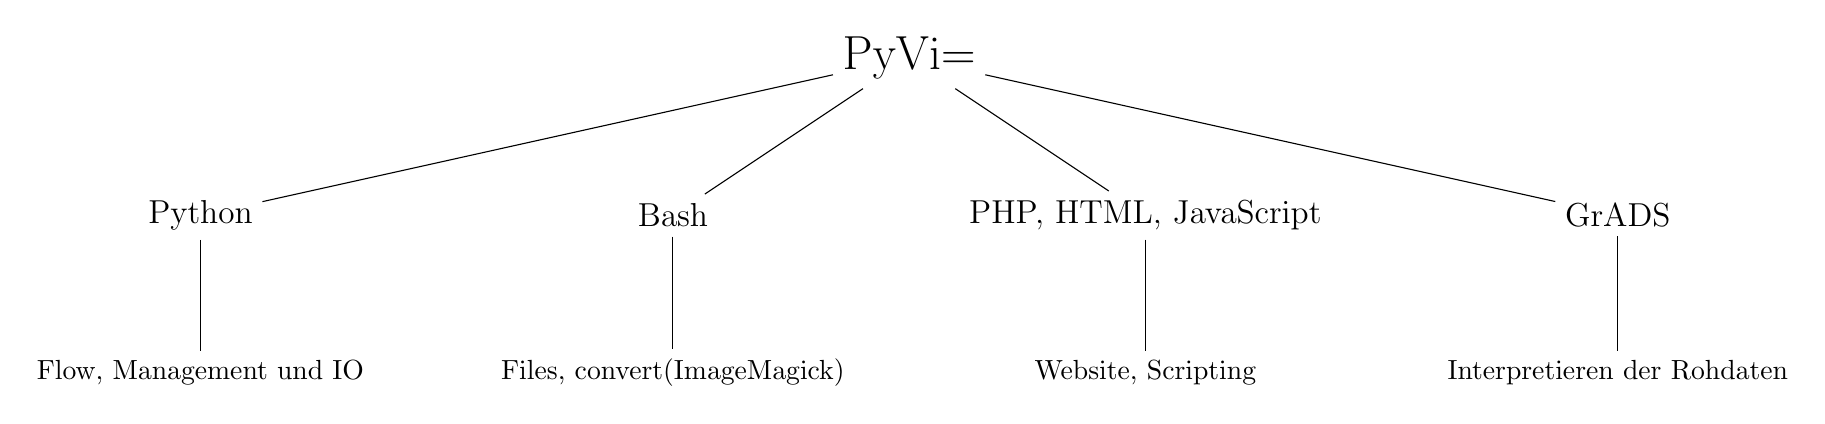
\begin{tikzpicture}[
every node/.style = {},
level 1/.style = {sibling distance = 6cm},
level distance = 2cm
]
\node {\LARGE PyVi$=$\vs}
    child { node {\large Python} 
    		child { node{Flow, Management und IO}}
    }
    child { node {\large Bash}
    		child { node {Files, convert(ImageMagick)}}
    }
    child { node {\large PHP, HTML, JavaScript}
    		child { node {Website, Scripting}}
    }
    child { node {\large GrADS} 
    		child { node{Interpretieren der Rohdaten}}
    };
\end{tikzpicture}
}
\end{center}
\label{fig:pyvi}
\caption{Benutzte Programmiersprachen}
\end{figure}

\subsubsection*{Hauptprogramm}
\lstinputlisting[language=Python,firstline=12, lastline=41,firstnumber=12,caption={,,Mainfunktion'' von \vs\ (auvi.py)}]{\pyvidir auvi.py}
\lstinputlisting[language=Python,caption={Konstanten (local.py)},firstline=3,lastline=7,firstnumber=3]{\pyvidir local.py}
\lstinputlisting[language=Python,caption={Hinzufügen von neuen Orten, Gebieten und Parametern (local.py)},firstline=11,lastline=28,firstnumber=11]{\pyvidir local.py}
\lstinputlisting[language=Python,caption={Routine zum schreiben von JSON Dateien (local.py)},firstline=30,lastline=41,firstnumber=30]{\pyvidir local.py}
\lstinputlisting[language=Python,caption={Datei In- und Output (filemanager.py)},firstline=39,lastline=66,firstnumber=39]{\pyvidir filemanager.py}
\lstinputlisting[language=Python,caption={Umwandeln von Konturplots in Gif Dateien (filemanager.py)},firstline=68,lastline=80,firstnumber=68]{\pyvidir filemanager.py}

\subsubsection*{JSON Definitionen}
Im folgenden Listing wird die Definition von Ortspunkten
\footnote{Ortspunkte stehen im Kontrast zur Gebietsdefinition. Gebiete werden durch minimale Breiten- und Höhengrade definiert und besitzen eine Breite und Höhe. Anwendungsbeispiel: Europa, Welt, Asien, ...} gezeigt.
Diese werden im JSON Format gespeichert.
Die Liste kann um beliebig viele andere Orte erweitert werden.
\lstinputlisting[language=json, caption={Beispielobjekte für Ortspunkte (locals.json)}]{\pyvidir locals.json}
In der Liste steht der erste String für den Ortsnamen. Der zweite Wert ist ein Double für den Breitengrad gefolgt vom Längengrad.
Da von den Orten auch ein Konturplot erzeugt werden soll wird mit dem 4. Wert abgespeichert wie groß die Übersichtskarte sein soll (In Grad um den Ort).
Der letzte Wert zur Definition eines Ortspunktes ist die Zeitdifferenz zur GMT Zeit.

\subsubsection*{GrADS Scripte}
\lstinputlisting[language=grads,caption={GrADS Routine zum erstellen allgemeiner Funktionsgraphen (line.gs)}]{\pyvidir grads/line.gs}
\lstinputlisting[language=grads,caption={GrADS Routine zum erstellen allgemeiner Konturplots (plot.gs)},label= code:plotgengs , firstline=104, lastline=115, firstnumber=104]{\pyvidir grads/plot.gs}
In Listing \ref{code:plotgengs} greifen wir auf verschiedene eigene Funktionen zurück um die Konturplotgrafiken zu füllen. Um der Ablauf des Skriptes zu verstehen werden wir die wichtigsten hier nun mit erläutern.
\lstinputlisting[language=grads,caption={Zeichnen der Achseneinteilung und Legende unter GrADS für Plots (plot.gs)}, firstline=117, lastline=136, firstnumber=117]{\pyvidir grads/plot.gs}
Die Variable $color$ spielt in diesem Teil des Skriptes eine große Rolle.
Diese Variable ist in diesem Kontext ein Pointer auf ein anderes GrADS Skript,
welches die Farbdefinitionen enthält.
Dieses Farbscript lässt sich leicht vom Computer nach den Eingaben eines Nutzers erzeugen.
% TODO Farbscript ersetzt durch Datenbank
\lstinputlisting[language=grads,firstline=8, lastline=28,caption={Beispiel Farbdefinition für Temperaturkonturplots (t2m.gs)},label=code:t2mcols]{\pyvidir grads/t2m.gs}
In Listing \ref{code:t2mcols} wird die Funktion gezeigt die bestimmten Zahlen eine Farbe zuweist.
Diese Farben sind im RGB Format codiert.
Die Definition ist so zu lesen:

\begin{lstlisting}[language=grads]
	'set rgb <num> <rot> <gruen> <blau>'
\end{lstlisting}

Die Farbwerte sind in einem Intervall von $0$ gar nicht vorhanden bis $255$ voller Kanal.
Um diese Farbwerte dann zu nutzen müssen diese noch den Wetterdaten zugewiesen werden.
Dieses geschieht unabhängig von den Einheiten im selben Script.
Auch hier kann der Text leicht von einem Computer generiert werden.
\footnote{Wenn wir davon sprechen, dass Daten vom Computer generiert werden ist gemeint, dass ein Nutzer der Website oder App seine Vorlieben mithilfe einer HTML-Form auswählt und von diesen Werten im Hintergrund eine Datei erzeugt.}


\subsubsection*{Webseite}
Das Front-End unserer Arbeit ist eine Website
\footnote{Diese Website kann auch in eine App gepackt werden, zur Veröffentlichung braucht man allerdings ein Entwicklerkonto bei Google oder Apple}.

Die Website ist programmiert in HTML (Hyper Text Markup Language), PHP (PHP\footnote{Rekursives Akronym}: Hypertext Preprocessor) und JavaScript.
Als Webserver benutzen wir Apache2 \cite{php} \cite{apache} \\

\subsubsection{Versionen}
Im Laufe der Arbeit entstanden mehrere lauffähige Versionen.
Diese beginnen mit puren GrADS-Scripten um überhaupt Grafiken zu erzeugen zu Beginn der Projektarbeit in 2013.
Um dieses Erzeugen zu automatisieren packten wir alle nötigen Befehle in eine BASH Datei.
Diese Bash Datei musste die Ordnerstruktur herstellen und kontrollieren.
Sie war außerdem in der Lage neue Versionen unserer Software zu erkennen und auf Befehlt vom Server zu laden.
Auf diese Version bauten wir auf,
nachdem wir sie bei dem Jugend Forscht Wettbewerb 2014 präsentierten und den zweiten Platz erreichten.\\
Um allerdings schnellere Ergebnisse zu erzielen übersetzte Markus das komplette Programm von Bash in Python.
Durch die modulare Struktur von Python können unsere Funktionen in andere Projekte als Bibliotek eingebunden werden.\\
Über Python können wir effektiver die Daten analysieren, können leichter komplexe Bedingungen kontrollieren und auch die Interaktion mit dem Nutzer ist erleichtert.
Durch Python und JSON konnten wir das Projekt dann vollständig automatisieren.

\subsubsection*{Git}
Ab Anfang 2015 benutzten wir eine neue Umgebung um an unserem Programmen und der Setzung zu arbeiten.
% TODO unabhängig von genutzten Mitteln GIT
Die Umgebung Git % FIXME Git Quelle!
ermöglicht im eigentlichen Sinne Programmierern gleichzeitig an einem Projekt kooperativ zu arbeiten.
Wir konnten diese Software zuerst auf dem eigenen Server und später zusätzlich auf der Website \link{GitHub.com} % FIXME GitHub Quelle
nutzen.
Der Git ,,Workflow'' ist auch ohne Internetverbindung komplett funktionstüchtig.
Wir machen Änderungen, verpacken sie und senden sie zum Server.
Dieses Änderungspacket erhält eine einzigartige Identifikation.
Durch diese Identifikation können wir auf jede einzelne Version unserer Software und Setzung zugreifen.
Zusätzlicher erreichen wir so eine hohe Datensicherheit und schnelle parallele Entwicklung mit gegenseitiger Kontrolle\footnote{Ziel ist es den Inhalt zu kontrollieren, nicht den Projektpartner}.

\subsubsection{genutzte Mittel} % AuVi Entwicklung
% Website, Server, ...
% Raspberry Pi x2
% Software: 	Linux -> Ubuntu, Debian, Raspbian
% 				Apache2, Git, Python2:3, PHP, SSH
% 				Editor SublimeText, Eclipse, Atom

\subsubsection{Servertechnik} % AuVi Entwicklung
% TODO Beschreibung Architektur, Ordnerstruktur
% NOTE z.B. /etc/apache2/sites-enabled/*
% NOTE Links, Domains, Websapce, ...
% Betreuung, Einarbeitung, ...

\subsection{Schnittstelle mit dem Nutzer} % AuVi
% TODO Defintion GUI, Zweck einer IO

\subsubsection{Webseite} % AuVi Schnittstelle
% Domain: viwetter.de
% Kosten: 7 EUR im Jahr, Server ist AuVi-Server
% TODO Übertrage Gerüst auf viwetter.de (Markus)
% Auf Server: /home/pi/viwetter.de/.
Die von uns gemacht Website um Ergebnisse anzuzeigen.

\subsubsection{Datenformate} % AuVi Schnittstelle
Da wir unsere erzeugten Grafiken auf einer Website und App darstellen wollen müssen wir sehr darauf achten,
dass die Dateiformate zum einen komprimiert genug sind um heruntergeladen werden zu können und zum anderen noch einen gewissen Qualitätsstandard behalten.\\
Außerdem sind Mobiltelefone nicht in der Lage alle Dateiformate anzuzeigen,
die ein Webbrowser auf einem Computer ohne Probleme handhabt.
Als die sichersten Dateiformate haben wir PNG und JPG für Bilder und GIF für Animationen auserkoren.
Wir haben lange versucht die Animationen als Video zu kodieren.
Allerdings bemerkten wir nur geringe Einsparungen in der Dateigröße und stellten gleichzeitig Anzeigeprobleme fest.

\subsubsection{Schulhompage} % AuVi Schnittstelle
Da wir ein Projekt des Schulzentrum Kühlungsborns sind (\link{http://www.schulzentrum-kborn.de}) sind wir auf dessen Seite unter ,,Lernen über Fächergrenzen'' als Campus Pro Projekt eingetragen \cite{szkb}.
Dort sind wir unter dem Titel ,,CaP \jf : Junge Atmosphären-forscher JAF'' aufzufinden.
Da die Bearbeitung der offiziellen Schulzentrum Kühlungsborn Seite sich als Umständlich aufzeigte,
richteten wir eine eigene Seite auf unserem Server ein.
Diese ist unter \link{http://team.viwetter.de}
für alle zu erreichen.
Diese Seite soll nicht die Ergebnisse unseres AuVi Programms widerspiegeln sondern dient als Webpräsenz des Projektes.

\subsection{Szenario} % AuVi
Wir werden nun Beispiele angeben, wie unser Programm genutzt werden kann.
Es gibt darüber hinaus sehr viele Möglichkeiten aus dem Programm individuellen Nutzen zu ziehen.

\subsubsection{Frühwarnung} % AuVi Szenario
% Nach dem Ampel System eigene Parameter die Gefährdung darstellen markieren. Z.B. Segler mit Windgeschwindigkeit auf Seelevel, Segelflieger mit Windgeschwindigkeit und Richtung auf x-Meter Höhe. Allgemeiner Arbeiter mit Temperatur.
Das von uns entwickelte System kann verwendet werden um wetterbedingte Gefahrensituationen frühzeitig zu erkennen.
Anhand der globalen Datenquellen und dem Hintergrund unseres Systems ist es einem Nutzer möglich für seinen Ort selbst die Parameter zu wählen die für Ihn eine Gefährdung darstellen.\\
Es ist uns wichtig, dass unsere Visualisierung keine Laien abschreckt,
deshalb haben wir uns entschieden die Frühwarnung in Form eines Ampelsystems an den Nutzer zu bringen.
Dieser kann bei Interesse an der Frühwarnfunktionalität eine Spanne angeben,
in der der entsprechende Parameter sicher ist (grün), gefährlich wird (gelb) oder gefährlich ist (rot).
Diese sehr visuelle Form soll dabei auf einem Blick ermöglichen die Wetterlage abzuschätzen.\\
Für detaillierte Auswertungen bieten wir andere Anzeigeformate an.

\subsubsection{Exotische Orte} % AuVi Szenario
Ob mitten im Ozean oder in der Wüste, unser Programm liefert Prognosen für jeden Ort.
Wir benötigen nur die dazugehörigen Koordinaten.
% TODO Wie wir an die Daten gelangen
Die Genauigkeit ist von der Zeitspanne und der Entfernung zur physikalischen Messstation abhängig.
Je weiter das Wetterereignis in der Zukunft liegt, desto geringer ist die Genauigkeit.
Die Genauigkeit steigt, wenn sich eine Messstation im näheren Umfeld befindet.

\subsubsection{Wissenschaft} % AuVi Szenario
Wissenschaftler können von uns bereitgestellte Parameter kombinieren und sich so neben allgemein komplexeren meteorologischen Daten auch besonders interessante meteorologische Ereignisse grafisch darstellen lassen.
Wenn jemand zum Beispiel Zusammenhänge zwischen der Ozonschicht und der Temperatur erforscht,
kann er sich eine Grafik ausgeben lassen, die ihm diese beiden Parameter darstellt.
% Dr. Eixmann fragen, was man sich wissenschaftlich visualisieren könnte
% TODO Plot einbinden

\subsubsection{Anpassung} % AuVi Szenario
Wie zuvor genannt kann der Nutzer eigene Muster einstellen und so das Programm erweitern.
Diese Möglichkeit erlaubt dem Nutzer diesem Service, den wir anbieten, um eigene Funktionen zu erweitern.
Ein Beispiel ist der Segler, der in einem Bestimmten Intervall von Windstärke und Windrichtung am besten seinen Sport ausüben kann.\\
Der Segler würde sich diese Parameter dann für das Gebiet seiner Interesse plotten lassen und kann dann noch Farben wählen.
Ähnlich wie das Frühwarnsystem kann er sich nun aber seine eigene Skala der ,,Eignung zum Segeln'' erstellen.
% TODO Verschiede Visualisierungen (der selben Daten)
% Inhalte für die besondere Lerleistung

\subsection{Öffentlichkeitsarbeit} % AuVi
% Messen, Vorträge, Dokumentation, Poster
Um unsere Arbeit zu präsentieren, entstanden im Laufe des Projekts mehrere Poster.
Anfangs entwickelten wir diese in PowerPoint, sind dann allerdings auf Gimp umgestiegen,
da sich das für unsere Arbeit vorteilhafter gestaltete.
Auf den Postern war meist zuerst eine kleine Einführung in das Projekt.
Danach schloss sich eine nähere Erläuterungen desselben an.
Um das Poster für den Betrachter attraktiver und anschaulicher zu machen,
stellten wir einige Themen in grafischer Form dar und veranschaulichten unsere Ergebnisse mit Beispielgrafiken. \\
Häufig wurde auch eine schriftliche Erläuterung des Projekts gefordert,
in der alles ausführlich erklärt wird.
Diese Dokumentation des Projekts schrieben wir in \LaTeX .
Auch in diesen Dokumentationen wurden Übersichten und Grafiken als Anschauungsmaterial beigefügt und nötigenfalls näher erläutert.\\
Solche Dokumentationen und Poster kamen zum Beispiel bei den Landeswettbewerben \jf in Rostock (Mecklenburg Vorpommern) zur Anwendung.
Bei diesem Wettbewerb werden aus dem gesamten Bundesland Projekte aus verschiedenen Fachgebieten präsentiert.
Es wird unterteilt in Arbeitswelt, Biologie, Chemie, Mathematik/Informatik, Geo- und Raumwissenschaften und Technik.
Die jeweils Erstplatzierten in jedem Bereich qualifizieren sich für den darauffolgenden Bundeswettbewerb.
Am Landeswettbewerb nahmen wir erstmalig 2013 teil.
Allerdings hatten wir uns erst kurz vorher zusammengefunden,
sodass wir das Projekt unserer Vorgänger vorstellten.
Wir nahmen am Wettbewerb teil um erste Erfahrungen zu sammeln und uns darüber klar zu werden,
wo wir einmal hin wollen.
Im darauf folgenden Jahr erreichten wir mit unserem Projekt ,,Auvi - Automatisierte Visualisierung von Wetterstations- und Wetterprognosedaten'' den zweiten Platz in der Kategorie Geo- und Raumwissenschaften.
Wir arbeiteten weiter an unserem Projekt und im Jahr 2015 gewannen wir den Landeswettbewerb sogar mit dem Projekt ,,AuVi - Automatisierte Visualisierung von meteorologischen Daten'' und qualifizierten uns so für den Bundeswettbewerb.\\
Wir nahmen auch an weiteren Veranstaltungen teil,
bei denen wir unser Projekt vorstellten.
Dazu gehört zum Beispiel der IHK-Schulpreis.
Im Jahr 2014 bewarb sich unsere Schule mit dem Projekt CampusPro.
Wir durften zusammen mit Vertretern aus anderen Projekten unsere Schule bei dieser Veranstaltung vertreten.
Im Jahr darauf nahmen wir wieder daran teil. Diesmal allerdings mit unserem Projekt an sich.\\
An unserer Schule wird die Möglichkeit geboten durch umfassende Projektarbeit ein IHK-Zertifikat zu erlangen.
Um dieses zu erlangen werden Vorträge gehalten, in denen das jeweilige Projekt präsentiert wird.
Im Jahr 2014 eröffneten wir solch eine Vortragsveranstaltung,
indem wir kurz unser neues Projekt vorstellten.
Im Jahr 2016 werden wir uns dann selbst um ein IHK-Zertifikat bemühen.
% TODO Mehr über Messenfeedback
